\documentclass[a4paper,11pt,oneside]{article}

\usepackage{amsmath,amssymb,epsfig}
\usepackage[T1]{fontenc}
\usepackage{ae,aecompl}
\usepackage{url}
\usepackage{epsfig}
\usepackage{subfigure}
\addtolength{\voffset}{-1cm}
\addtolength{\hoffset}{-1cm}
\setlength{\parindent}{0in}
\addtolength{\textwidth}{1.8cm}
\addtolength{\textheight}{1cm}
\addtolength{\parskip}{.5cm}

% Example definitions.
% --------------------
\def\e{{e^{j\omega}}}
\def\W{{W_M}}
\def\sumk{{\sum_{k=-\infty}^{\infty}}}
\def\x{{\mathbf x}}
\def\X{{\mathbf X}}
\def\Y{{\mathbf Y}}
\def\u{{\mathbf u}}
\def\U{{\mathbf U}}
\def\x{{\mathbf x}}
\def\s{{\mathbf s}}
\def\A{{\mathbf A}}
\def\y{{\mathbf y}}
\def\w{{\mathbf w}}
\def\B{{\mathbf B}}
\def\a{{\mathbf a}}
\def\D{{\mathbf D}}
\def\P{{\mathbf P}}
\def\n{{\mathbf n}}
\def\V{{\mathbf V}}
\def\R{{\mathbf R}}
\def\I{{\mathbf I}}
\def\M{{\mathbf M}}
\def\sech{{\mathrm{sech}}}
\def\L{{\cal L}}
\def\Cum{{\rm{Cum}}}
\def\var{{\rm{var}}}
\def\T{{\mathbf T}}
\def\C{{\mathbf C}}
\def\tf{{\emph{t-f}}}


% Title.
% ------
\title{\large{\textbf{EXERCISE 2}}}
\author{SGN-1156 Signal Processing Techniques\\
\texttt{http://www.cs.tut.fi/courses/SGN-1156}\\
Tampere University of Technology\\
Germ\'an G\'omez-Herrero, \url{http://germangh.com}}
\date{December 4, 2009}


\begin{document}

\maketitle


\textbf{Important:} The most important information of Chapter 3 of the book is in tables 3.1, 3.2 and specially 3.3 and 3.4. When computing DTFTs it is often useful to know that:

\[
\sum_{n=m}^{k}r^{n}=\frac{r^{k+1}-r^m}{r-1}
\]

Note that I made a mistake when writing the expression above in the whiteboard. Thanks to Junsheng for reporting this. Other useful sums are:

\[
\sum_{n=0}^{\infty} r^{n}=\frac{1}{1-r} \qquad |r|<1
\] 

\[
\sum_{n=0}^{\infty} nr^{n}=\frac{r}{(1-r)^2} \qquad |r|<1
\]

Remember also the relationships:

\[
\cos \omega = \frac{e^{j\omega}+e^{-j\omega}}{2}
\]

\[
\sin \omega = \frac{e^{j\omega}-e^{-j\omega}}{2j}
\]






%%%%%%%%%%%%%%%%%%%%%%%%%%%%%%%%%%%%%%%%%%%%%%%%%%%%%%%%%%%%%%%
\textbf{PROBLEM 1:} Determine the DTFT of each of the following sequences:

\begin{itemize}
\item[(a)] $x_a[n] = \mu[n]-\mu[n-5]$
\item[(b)] $x_b[n] = \alpha^n\left(\mu[n]-\mu[n-8]\right) \qquad |\alpha|< 1$
\item[(c)] $x_c[n] = (n+1)\alpha^n\mu[n] \qquad |\alpha|<1$
\end{itemize}  



\vspace{1cm}
%%%%%%%%%%%%%%%%%%%%%%%%%%%%%%%%%%%%%%%%%%%%%%%%%%%%%%%%%%%%%%%



%%%%%%%%%%%%%%%%%%%%%%%%%%%%%%%%%%%%%%%%%%%%%%%%%%%%%%%%%%%%%%%
\textbf{SOLUTION:}
There are two ways of computing the DTFT of a sequence. Either you apply directly the formula of the DTFT or you try to express your sequence as a linear combination of elementary sequences for which you know the DTFT. 

\vspace{.5cm}

\textbf{(a)}

Using directly the DTFT formula:

\[
X_a(e^{j\omega})=\sum_{n=0}^{\infty}x_a[n]e^{-j\omega n}=\sum_{n=0}^{4}e^{j\omega n}=\frac{e^{-j\omega 5}-1}{e^{-j\omega}-1}
\]

Using the fact that the DTFT of the unit step function is:

\[
\mu[n]\stackrel{DTFT}{\rightarrow} G(e^{j\omega})=\frac{1}{1-e^{-j\omega}}+\sum_{k=-\infty}^{\infty}\pi \delta(\omega+2\pi k)
\]

then:

\[ 
X_a(e^{j\omega})=G(e^{j\omega})-e^{-j\omega 5}G(e^{j\omega})=\frac{1-e^{-j\omega 5}}{1-e^{-j\omega}}-\underbrace{(1-e^{-j\omega 5})\sum_{k=-\infty}^{\infty}\pi \delta(\omega+2\pi k)}_{=0 \; \forall \omega}
\]

So we finally obtain:

\[ 
X_a(e^{j\omega})=\frac{1-e^{-j\omega 5}}{1-e^{-j\omega}}
\]

\vspace{.5cm}



\textbf{(b)}

\[
X_b(e^{j\omega})=\frac{1-\alpha^8 e^{-j\omega 8}}{1-\alpha e^{-j\omega}}
\]


\vspace{.5cm}
\textbf{(c)}

\[
X_c(e^{j\omega})=\frac{1}{(1-\alpha e^{-j\omega})^2}
\]
\vspace{1cm}
%%%%%%%%%%%%%%%%%%%%%%%%%%%%%%%%%%%%%%%%%%%%%%%%%%%%%%%%%%%%%%%


%%%%%%%%%%%%%%%%%%%%%%%%%%%%%%%%%%%%%%%%%%%%%%%%%%%%%%%%%%%%%%%
\textbf{PROBLEM 2: (problem 3.41 from the book)} Let $G_1(e^{j\omega})$ denote the discrete-time Fourier transform of the sequence $g_1[n]$ shown in the figure below. Express the DTFTs of $g_2[n]$, $g_3[n]$ and $g_4[n]$ in terms of $G_1(e^{j\omega})$. Do not evaluate $G_1(e^{j\omega})$.


\begin{figure}[ht!]
\centering
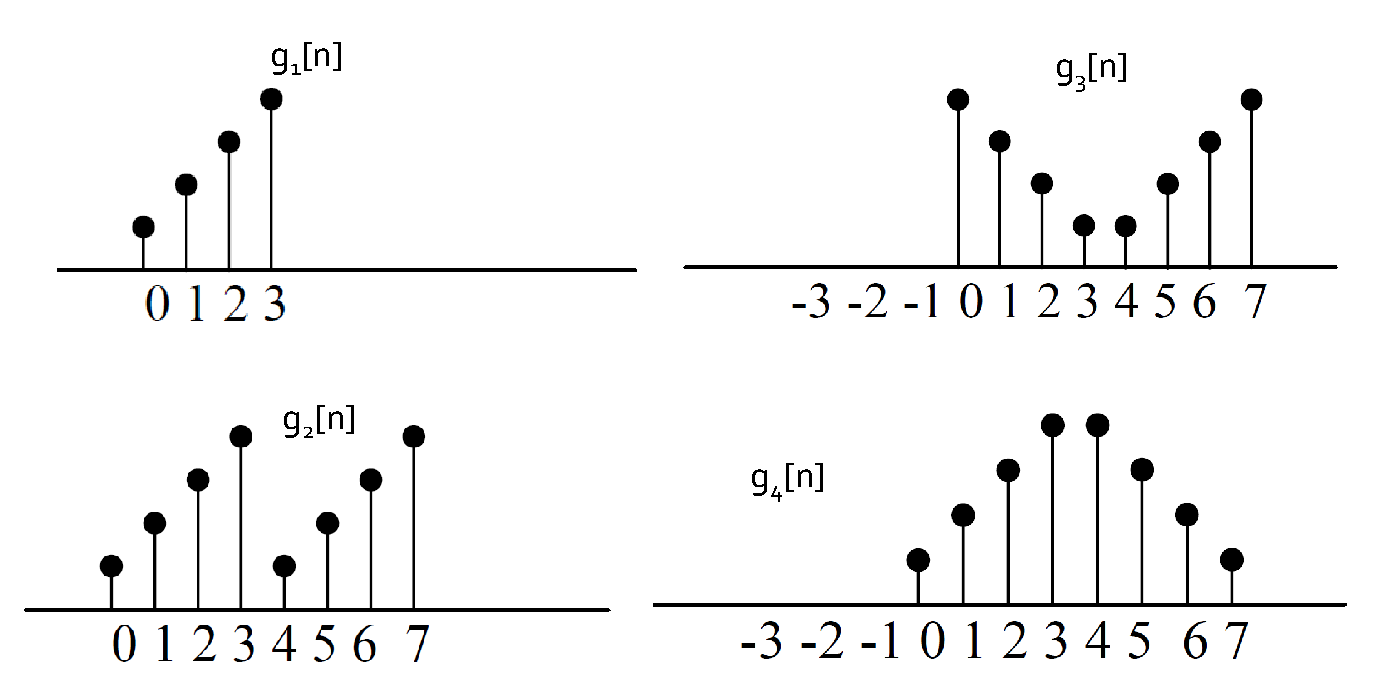
\includegraphics[width=.8\textwidth]{fig4.eps}
\end{figure}


\vspace{1cm}
%%%%%%%%%%%%%%%%%%%%%%%%%%%%%%%%%%%%%%%%%%%%%%%%%%%%%%%%%%%%%%%



%%%%%%%%%%%%%%%%%%%%%%%%%%%%%%%%%%%%%%%%%%%%%%%%%%%%%%%%%%%%%%%
\textbf{SOLUTION:}


$g_2[n]=g_1[n]+g_1[n-4]\Rightarrow G_2{e^{j\omega}}=\left(1+e^{-4j\omega}\right)G_1(e^{j\omega})$

\vspace{.5cm}

$g_3[n]=g_1[-(n-3)]+g_1[n-4]\Rightarrow G_3{e^{j\omega}}=e^{-j3\omega}G_1(e^{-j\omega})+e^{-j4\omega}G_1(e^{j\omega})$

\vspace{.5cm}

$g_4[n]=g_1[n]+g_1[-(n-7)]\Rightarrow G_4(e^{j\omega})=G_1(e^{j\omega})+e^{-j7\omega}G_1(e^{-j\omega})$

\vspace{1cm}
%%%%%%%%%%%%%%%%%%%%%%%%%%%%%%%%%%%%%%%%%%%%%%%%%%%%%%%%%%%%%%%



%%%%%%%%%%%%%%%%%%%%%%%%%%%%%%%%%%%%%%%%%%%%%%%%%%%%%%%%%%%%%%%
\textbf{PROBLEM 3:}  Consider the following interconnection of linear shift-invariant systems:

\begin{figure}[ht!]
\centering
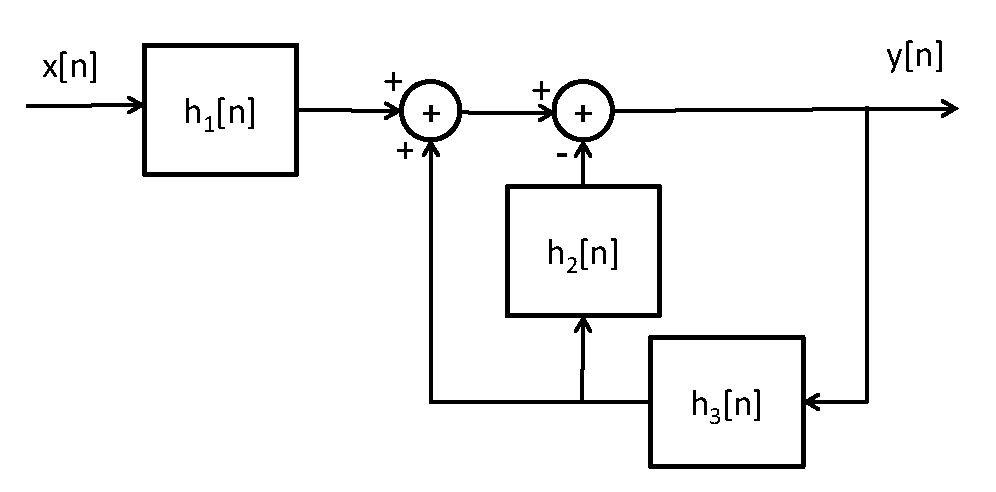
\includegraphics[width=.7\textwidth]{fig1.eps}
\end{figure}

Express the frequency response of the overall system $H(e^{j\omega})$ in terms of the frequency responses of the subsystems $H_1(e^{j\omega})$, $H_2(e^{j\omega})$, and $H_3(e^{j\omega})$.

\vspace{1cm}
%%%%%%%%%%%%%%%%%%%%%%%%%%%%%%%%%%%%%%%%%%%%%%%%%%%%%%%%%%%%%%%
\textbf{SOLUTION:}



The first step is to represent the given system in frequency domain and to introduce new intermidiate variables in any interconnection between diagram elements. This is shown below:


\begin{figure}[h!]
\centering
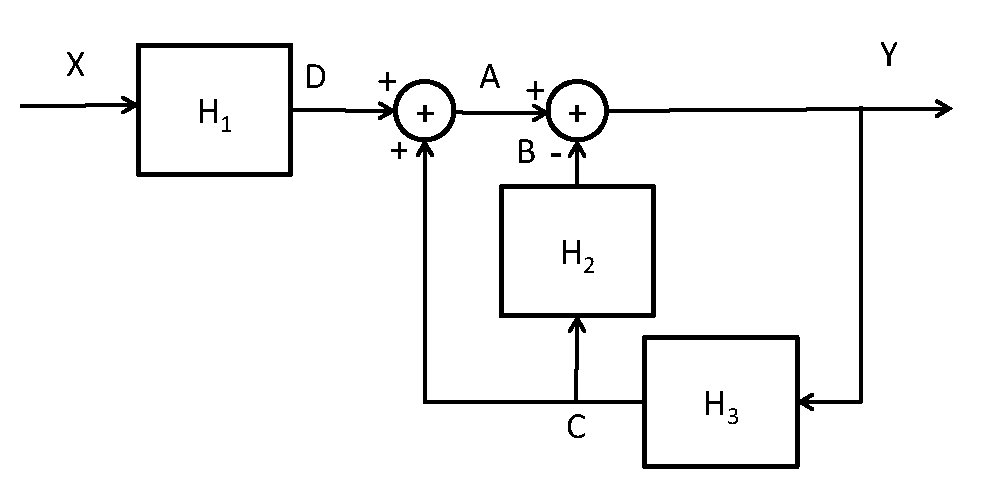
\includegraphics[width=.7\textwidth]{fig2.eps}
\end{figure}

For simplicity we have omitted all the terms $(e^{j\omega})$ in the diagram above. Unless otherwise stated uppercase letters will denote Fourier-domain variables and lower-case letters time-domain ones. We can now write all the system equations in Fourier domain:

\begin{eqnarray}
Y &=& A-B\label{eq1}\\
A &=& D+C\label{eq2}\\
B &=& H_2\cdot C\label{eq3}\\
C&=&H_3\cdot Y\label{eq4}\\
D&=&H_1 \cdot X\label{eq5}
\end{eqnarray}

The overall frequency response is defined as $H=\frac{Y}{X}$. Therefore, we need to combine the five equations above into a single one that has only $X$ and $Y$ as unknowns. Combining Eqs.~\ref{eq1},~\ref{eq2} and~\ref{eq3} we obtain:

\begin{equation}\label{eq6}
Y = D + (1-H_2)C
\end{equation}

Now combining Eq.~\ref{eq6} with Eqs.~\ref{eq4} and~\ref{eq5} we get to:

\begin{equation}\label{eq7}
Y = H_1\cdot X + (1-H_2)H_3 Y
\end{equation}

which has only two unknowns: $X$ and $Y$. Reorganizing Eq.~\ref{eq7} we finally obtain the overall frequency response of the system:

\begin{equation}
Y = \frac{H_1}{1+H_3(H_2-1)}X \Rightarrow H(e^{j\omega})=\frac{Y(e^{j\omega})}{X(e^{j\omega})}=\frac{H_1(e^{j\omega})}{1+H_3(e^{j\omega})(H_2(e^{j\omega})-1)}
\end{equation}



\vspace{1cm}
%%%%%%%%%%%%%%%%%%%%%%%%%%%%%%%%%%%%%%%%%%%%%%%%%%%%%%%%%%%%%%%







%%%%%%%%%%%%%%%%%%%%%%%%%%%%%%%%%%%%%%%%%%%%%%%%%%%%%%%%%%%%%%%
\textbf{PROBLEM 4.} Consider the following interconnection of LTI systems:

\begin{figure}[ht!]
\centering
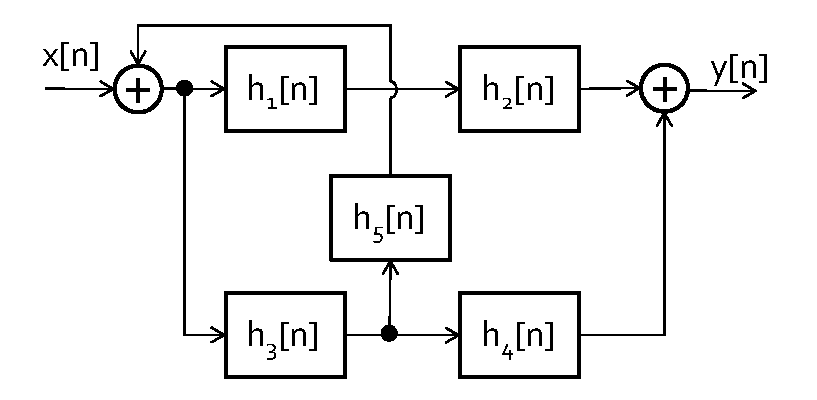
\includegraphics[width=.7\textwidth]{fig3.eps}
\end{figure}

Express the frequency response of the overall system $H(e^{j\omega})$ in terms of the frequency responses of the subsystems depicted in the diagram.

\vspace{1cm}
%%%%%%%%%%%%%%%%%%%%%%%%%%%%%%%%%%%%%%%%%%%%%%%%%%%%%%%%%%%%%%%
 
%%%%%%%%%%%%%%%%%%%%%%%%%%%%%%%%%%%%%%%%%%%%%%%%%%%%%%%%%%%%%%%
\textbf{SOLUTION:}

The first thing that we do is to transform all variables to the DTFT domain (we omit the $e^{j\omega}$ terms), to introduce intermediate variables in every connection between system elements and to simplify as much as possible the diagram:

\begin{figure}[ht!]
\centering
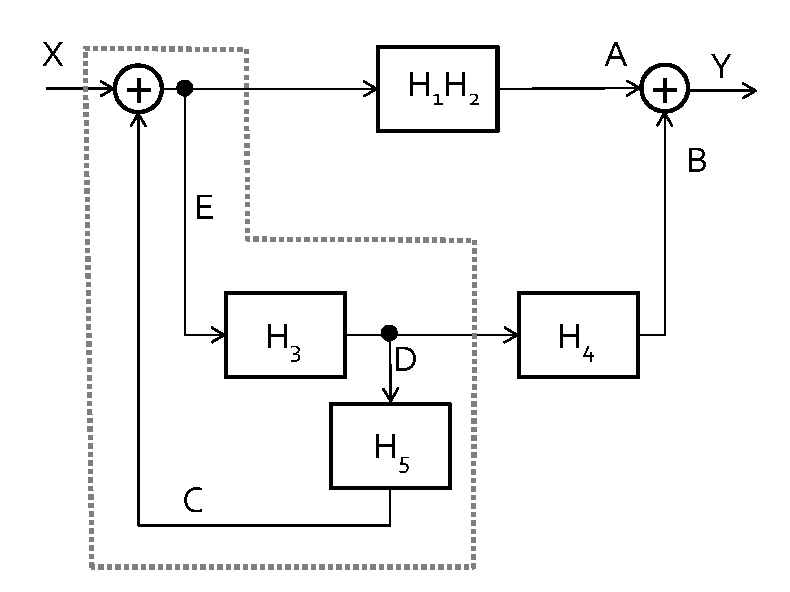
\includegraphics[width=.7\textwidth]{fig6.eps}
\end{figure}

We can observe that there is a feedback loop involving the first addition operator and systems $H_3$ and $H_5$ (surrounded by a dashed line in the diagram above). The best way to proceed is to first compute the frequency response of the sub-system bounded by the dashed line, i.e. to find the relationship between $D$ and  $X$. We can see that the feedback sub-system contains 4 unknowns ($X$, $E$, $D$, $C$) which means that we will need to write 3 equations:

\begin{eqnarray}
D &=&H_3E\label{eq:d}\\
C &=&H_5 D\label{eq:c}\\
E &=&X+C\label{eq:e}
\end{eqnarray}

Combining these three equations:

\[
D = H_3X + H_3C = H_3X+H_3H_5D\Rightarrow D = \frac{H_3}{1-H_3H_5}X
\]

Then we can also find the relationship between $E$ and the input $X$:

\[
D = H_3E \Rightarrow E=\frac{D}{H_3} =\frac{1}{1-H_3H_5}X
\]

Now we can proceed to determine the overall frequency response of the whole system. Since in the whole system we have 7 unknowns, we need 6 equations to fully determine the output with respect to the input. We already wrote 3 equations above so we just need 3 more:

\begin{eqnarray}
Y &=&A+B\\
A &=&H_1H_2E\\
B &=&H_4D
\end{eqnarray}

Combining the three equations above:

\[
Y = A+B=H_1H_2E+H_4D
\]

and using the expressions that we found for $E$ and $D$ with respect to $X$:

\[
Y =H_1H_2E+H_4D= \frac{H_1H_2+H_4H_3}{1-H_3H_5}X
\]


\vspace{1cm}
%%%%%%%%%%%%%%%%%%%%%%%%%%%%%%%%%%%%%%%%%%%%%%%%%%%%%%%%%%%%%%%




%%%%%%%%%%%%%%%%%%%%%%%%%%%%%%%%%%%%%%%%%%%%%%%%%%%%%%%%%%%%%%%
\textbf{PROBLEM 5.} Consider the interconnection of linear shift-invariant systems in the figure below:



\begin{figure}[h!]
\centering
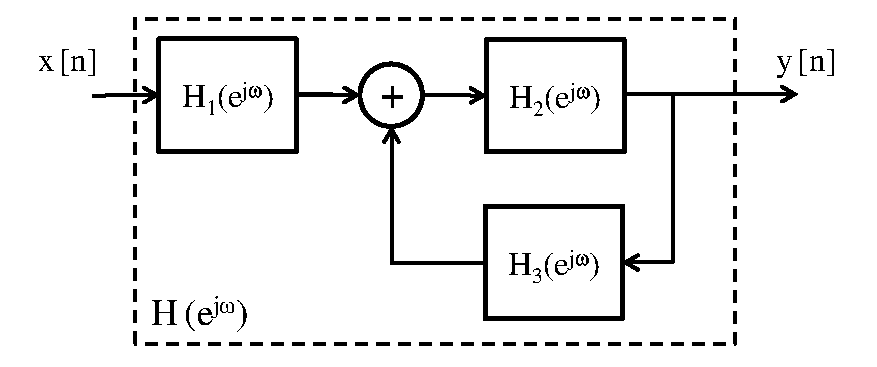
\includegraphics[width=.7\textwidth]{fig5.eps}
\end{figure}



\begin{itemize}
\item[(a)] Express the frequency response of the overall system $H(e^{j\omega})$ in terms of the frequency responses of the subsystems $H_1(e^{j\omega})$, $H_2(e^{j\omega})$ and $H_3(e^{j\omega})$.
\item[(b)] Determine the frequency response $H(e^{j\omega})$ of the overall system if:
\[
\begin{array}{lll}
h_1[n] &=& \frac{\sin(\frac{\pi}{3}n)}{\pi n}\\
h_2[n] &=&(0.3)^{n}\mu[n]\\
h_3[n] &=&\delta[n-2]
\end{array}
\]
\end{itemize}


\vspace{1cm}
%%%%%%%%%%%%%%%%%%%%%%%%%%%%%%%%%%%%%%%%%%%%%%%%%%%%%%%%%%%%%%%
 
%%%%%%%%%%%%%%%%%%%%%%%%%%%%%%%%%%%%%%%%%%%%%%%%%%%%%%%%%%%%%%%
\textbf{SOLUTION:}

The overall frequency response is:

\[
Y = \frac{H_1H_2}{1-H_2H_3}X \Rightarrow H=\frac{H_1H_2}{1-H_2H_3}
\]

Transforming $h_1[n]$, $h_2[n]$, $h_3[n]$ to the DTFT domain we finally obtain that:

\[
H(e^{j\omega}) = \left\{
\begin{array}{lll}
\frac{1}{1-0.3e^{-j\omega}-e^{-j\omega 2}}&\qquad& |\omega|\leq\omega_c\\
0 &\qquad&|\omega|>\omega_c
\end{array}
\right.
\]


\vspace{1cm}
%%%%%%%%%%%%%%%%%%%%%%%%%%%%%%%%%%%%%%%%%%%%%%%%%%%%%%%%%%%%%%%




%%%%%%%%%%%%%%%%%%%%%%%%%%%%%%%%%%%%%%%%%%%%%%%%%%%%%%%%%%%%%%%
\textbf{PROBLEM 6 (problem 3.59 from the book):} An LTI IIR discrete-time system is described by the difference equation
\[
y[n] + a_1y[n-1] = b_0x[n]+b_1x[n-1]
\]
where the input is $x[n]$, the output is $y[n]$, and the constants $a_1$, $b_0$ and $b_1$ are real. Determine the expression for its frequency response. For what values of $b_0$ and $b_1$ will the magnitude response be a constant for all values of $\omega$?.




\vspace{1cm}
%%%%%%%%%%%%%%%%%%%%%%%%%%%%%%%%%%%%%%%%%%%%%%%%%%%%%%%%%%%%%%%



%%%%%%%%%%%%%%%%%%%%%%%%%%%%%%%%%%%%%%%%%%%%%%%%%%%%%%%%%%%%%%%
\textbf{SOLUTION:}
In order to obtain the frequency response of the system, first we need to transform the system's equation into the frequency domain:

\[
Y(e^{j\omega})+a_1e^{-j\omega}Y(e^{j\omega})=b_0X(e^{j\omega})+b_1e^{-j\omega}X(e^{j\omega})
\]

so the frequency response of the system is:

\[
H(e^{j\omega})=\frac{Y(e^{j\omega})}{X(e^{j\omega})}=\frac{b_0+b_1e^{-j\omega}}{1+a_1e^{-j\omega}}
\]

It is difficult to operate with the requirement $|H(e^{j\omega})|=K=\textrm{constant}$ due to the presence of complex quantities inside the absolute value operator. In order to get rid of complex terms the easiest is to solve for the equivalent requirement $|H(e^{j\omega}))|^2=K^2=\textrm{constant}$:

\[
\begin{array}{lll}
|H(e^{j\omega})|^2&=&H(e^{j\omega})H^*(e^{j\omega})=\frac{(b_0+b_1e^{-j\omega})(b_0+b_1e^{j\omega})}{(1+a_1e^{-j\omega})(1+a_1e^{j\omega})}\\
\\
&=&\frac{b_0^2+b_1^2+b_0b_1\left(e^{j\omega}+e^{-j\omega}\right)}{1+a_1^2+a_1\left(e^{j\omega}+e^{j\omega}\right)}=\frac{b_0^2+b_1^2+2b_0b_1\cos\omega}{1+a_1^2+2a_1\cos\omega}=K^2=C
\end{array}
\]

Then we have to find the values of $a_1$, $b_0$ and $b_1$ satifying:

\[
\underbrace{b_0^2+b_1^2}_{A}+\underbrace{2b_0b_1}_{B}\cos\omega = \underbrace{C+Ca_1^2}_{A'}+\underbrace{2Ca_1}_{B'}\cos\omega
\]

We can see that the expressions at each side of the equation above corresponds to a scaled sinusoid with non-zero mean. So we can enforce the equality by simply enforcing that the mean of the sinusoids is the same ($A=A'$) and that the scale of both sinusoids is also the same ($B=B'$):

\[
\begin{array}{lll}
A = A' &\Rightarrow & b_0^2+b_1^2 = C+Ca_1^2\\
B = B' &\Rightarrow & b_0b_1 = Ca_1\\
\end{array}
\]

Putting both equations together:

\[
b_0=C\frac{a_1}{b_1}\Rightarrow \frac{C^2a_1^2}{b_1^2}+b_1^2=C+Ca_1^2\Rightarrow b_1^4-C(1+a_1^2)b_1^2+C^2a_1^2=0
\]

The quadratic equation above has two solutions:

\[
b_1^2=\frac{C(1+a_1^2)\pm \sqrt{C^2(1+a_1^2)^2-4C^2a_1^2}}{2}
\]

Operating we get that the solution is either $b_1=\pm K$ or $b_1=\pm Ka_1$. We first try the former solution to check if it fulfills our requirement:

\[
|H(e^{j\omega})|=\left|\frac{\pm K a_1\pm Ke^{-j\omega}}{1+a_1e^{-j\omega}}\right|=K\left|\frac{a_1+ e^{-j\omega}}{1+a_1e^{-j\omega}}\right|
\]

Clearly, the expression above is not equal to a constant in general so this is not a valid solution of the problem. We try now the solution $b_1=\pm Ka_1$:


\[
|H(e^{j\omega})|=\left|\frac{\pm K \pm Ka_1e^{-j\omega}}{1+a_1e^{-j\omega}}\right|=K\left|\frac{1+ a_1e^{-j\omega}}{1+a_1e^{-j\omega}}\right|=K
\]

And therefore $b_1=\pm Ka_1$ is the solution that we need. The reason for one of the solutions that we found to be invalid is that we substituted the original requirement $|H(e^{j\omega})|=K$ for the alternative requirement $|H(e^{j\omega})|^2=K^2$. This had the effect of introducing an spurious solution since the latter equality is fulfilled not only when $|H(e^{j\omega})|=K$ but also when $|H(e^{j\omega})|=-K$. Obviously, the latter solution is not valid.

\vspace{1cm}
%%%%%%%%%%%%%%%%%%%%%%%%%%%%%%%%%%%%%%%%%%%%%%%%%%%%%%%%%%%%%%%



%%%%%%%%%%%%%%%%%%%%%%%%%%%%%%%%%%%%%%%%%%%%%%%%%%%%%%%%%%%%%%%
\textbf{PROBLEM 7:} Consider the system defined by the difference equation 

\[
y[n] = ay[n-1]+bx[n]+x[n-1]
\]

where $a$ and $b$ are real, and $|a|<1$. Find the relationship between $a$ and $b$ that must exist if the frequency response is to have a constant magnitude for all $\omega$, that is $|H(e^{j\omega})|=1$.
\vspace{1cm}
%%%%%%%%%%%%%%%%%%%%%%%%%%%%%%%%%%%%%%%%%%%%%%%%%%%%%%%%%%%%%%%



%%%%%%%%%%%%%%%%%%%%%%%%%%%%%%%%%%%%%%%%%%%%%%%%%%%%%%%%%%%%%%%
\textbf{SOLUTION:}
In order to obtain the frequency response of the system, first we need to transform the system's equation into the frequency domain:

\[
Y(e^{j\omega})=ae^{-j\omega}Y(e^{j\omega})+bX(e^{j\omega})+e^{-j\omega}X(e^{j\omega})
\]

so the frequency response of the system is:

\[
H(e^{j\omega})=\frac{Y(e^{j\omega})}{X(e^{j\omega})}=\frac{b+e^{-j\omega}}{1-a\cdot e^{-j\omega}}
\]

If the equality $|H(e^{j\omega})|=1$ hold then it must also hold the equality $|H(e^{j\omega})|^2=1$. Solving this latter equality is easier because the expression on the left side has only real terms inside the absolute value operator. Operating a bit:

\[
|H(e^{j\omega})|^2=1 \Longrightarrow H(e^{j\omega})\cdot H^*(e^{j\omega})=1
\]

substituting the value of $H(e^{j\omega})$ into the expression above we obtain:

\[
H(e^{j\omega})\cdot H^*(e^{j\omega})=\frac{(b+e^{-j\omega})\cdot (b+e^{j\omega})}{(1-a\cdot e^{-j\omega})\cdot(1-a\cdot e^{j\omega})}=\frac{1+b^2+b\cdot(e^{j\omega}+e^{-j\omega})}{1+a^2-a\cdot(e^{j\omega}+e^{-j\omega})}=1
\]

So, the numerator and denominator of the fraction above must be equal, which translates into the two equations:

\[
\begin{array}{lll}
1+b^2&=&1+a^2\\
b &=& -a
\end{array}
\]

Clearly, if and only if $b=-a$ the two equations are fullfiled and $|H(e^{j\omega})|^2=1$. Since we have only a single solution to the squared version of our original condition we can conclude that this solution has to be also the solution to our original constraint. That is $|H(e^{j\omega})|=1$ if and only if $b=-a$.

\vspace{1cm}
%%%%%%%%%%%%%%%%%%%%%%%%%%%%%%%%%%%%%%%%%%%%%%%%%%%%%%%%%%%%%%%



\end{document}